\chapter{Aplicação da programação linear na separação de pontos}

Na tarefa onde o obejtivo é a separação de dois ou mais conjuntos de pontos, sendo que cada conjunto representa um padrão, busca-se um método para que essa separação seja obtida com resultado ótimo. Cada conjunto é o resultado de um conjunto de pontos e cada ponto é é representado por um vetor de características.
Em \cite{Bennett92robustlinear} é proposto um modelo de programação linear capaz de um gerar um hiperplano de minimiza a soma dos pontos classificados de forma errada. Dessa forma o modelo é capaz de gerar um hiperplano separador para pontos linearmente separáveis e para conjutnos linearmente inseparáveis, o modelo gera o melhor hiperplano de forma que essa média calculada seja mínima. Na figura abaixo estão ilustrados os casos de dois conjuntos linearmente separáveis e dois conjuntos linearmente inseparáveis. COLOCAR FIGURA!!!
 
\begin{figure}
\centering
\subfigure[]{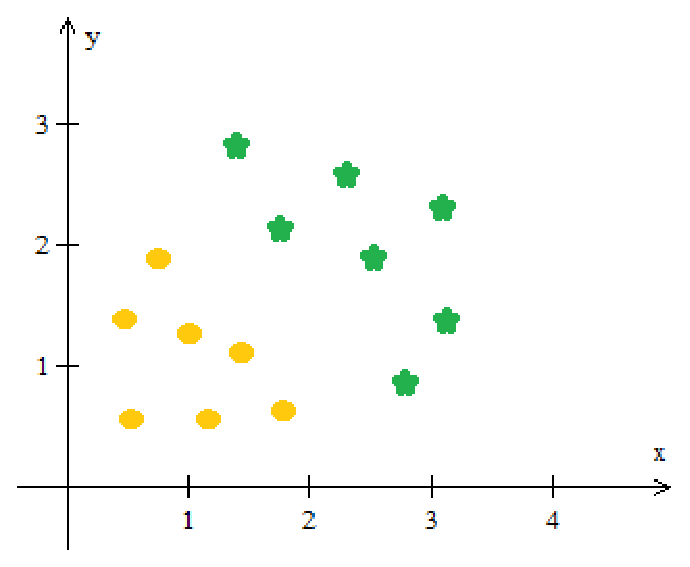
\includegraphics[scale=0.5]{graficos/linear_sepa}\label{fig1}}
\qquad
\subfigure[]{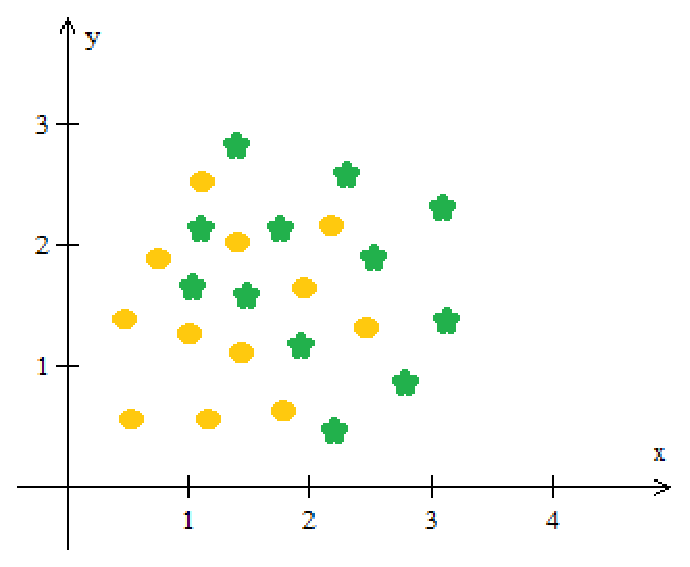
\includegraphics[scale=0.5]{graficos/linear_insepa}\label{fig2}}
\label{img:linear_sepa}
\caption{Em \ref{fig1} são apresentados dois conjuntos linearmente separáveis e em \ref{fig2} são apresentados dois conjuntos linearmente inseparáveis}
\end{figure}

\section{O modelo}
Considerando dois conjuntos, no espaço n-dimensional $ R^{n} $, sendo o conjunto A representado pela matriz m x n, e o conjunto B representado pela matriz k x n. Contextualizando, k e m são as quantidades de pontos em cada conjunto, e n é a quantidade de características. O modelo gera um hiperplano que separa os pontos dos dois conjuntos. De forma que os m pontos do conjunto A fiquem de um lado do hiperplano e os k pontos do conjunto B fiquem do outro lado do hiperplano. Na figura abaixo o modelo é apresentado. E a seguir é apresentado de forma mais detalhada.

$Min\ \frac{e^{t}y}{m} + \frac{e^{t}z}{k}\\
\ subject\ to  \\
\              -A\omega + e\gamma + e <= y\\
\              B\omega - e\gamma + e <= z\\
\              y>= 0, z>= 0 $

